\section{Anexos}
\subsection{Distribución de estratos socioeconómicos}
\begin{table}[htpb!]
\small
\centering
\scalebox{0.75}{
	\begin{tabular}{|c|c c c c c| c c c c c | c|}
	\hline
	\multicolumn{12}{|c|}{\textbf{ZONA NORTE}}\\
	\hline
	\multicolumn{1}{|c|}{\textbf{I Región}}\\
	\hline
	& \blue{ABC1} & \blue{C2} & \blue{C3} & \blue{D} & \blue{E} & \green{ABC1} & \green{C2} & \green{C3} & \green{D} &  \green{E} & \red{TOTAL} \\
	\hline
	Arica & 4,8\% & 18,0\% & 27,8 & 40,2\% & 9,2\% & 8.377 & 31.539 & 48.819 & 70.490 & 16.226 & \textbf{175.441} \\ 
	Iquique & 9,5\% & 25,7\% & 28,4\% & 31,1\% & 5,3\% & 15.638 & 42.309 & 46.642 & 51.170 & 8.641 & \textbf{164.396} \\
	Otras (4 comunas) & 0,6\% & 7,7\% & 24,7\% & 53,2\% & 13,7\% & 378 & 4.903 & 15.640 & 33.681 & 8.699 & \textbf{63.301} \\
	\hline
	\blue{Total Región} & 6,0\% & 19,5\% & 27,6\% & 38,5\% & 8,3\% & 24.388 & 78.741 & 111.101 & 155.341 & 33.566 & \textbf{\blue{403.138}}\\
	\hline
	\green{Total Región/País} & 2,4\% & 3,4\% & 3,6\% & 3,07\% & 1,86\% & 24.388 & 78.741 & 111.101 & 155.341 & 33.566 & \textbf{\blue{403.138}}\\
	\hline
	\multicolumn{1}{|c|}{\textbf{II Región}}\\
	\hline
	Antofagasta & 9,2\% & 21,7\% & 27,0\% & 35,4\% & 6,7\% & 27.212 & 64.102 & 79.970 & 104.767 & 19.741 & \textbf{295.792}\\
	Calama & 8,3\% & 24,1\% & 26,6\% & 34,0\% & 6,9\% & 11.356 & 32.929 & 36.402 & 46.421 & 9.493 & \textbf{136.600} \\
	Otras (5 comunas) & 2,2\% & 11,6\% & 25,4\% & 48,5\% & 12,3\% & 1.122 & 5.835 & 12.735 & 24.311 & 6.151 & \textbf{50.154} \\
	\hline
	\blue{Total Región} & 8,2\% & 21,3\% & 26,8\% & 36,4\% & 7,3\% & 39.689 & 102.866 & 129.108 & 175.498 & 35.385 & \textbf{\blue{482.546}}\\
	\hline
	\green{Total Región/País} &4,0\% &4,7\% &4,1\% &3,4\% &1,9\% & 39.689 & 102.866 & 129.108 & 175.498 & 35.385 & \textbf{\blue{482.546}}\\
	\hline
	\multicolumn{1}{|c|}{\textbf{III Región}}\\
	\hline
	Copiapo & 5,6\% & 15,8\% & 23,6\% & 41,5\% & 13,5\% & 7.115 & 19.862 & 29.717 & 52.314 & 16.976 & \textbf{125.983} \\
	Vallenar & 3,1\% & 10,4\% & 20,4\% & 43,3\% & 22,7\% & 1.348 & 4.566 & 8.936 & 18.962 & 9.938 & \textbf{43.750} \\
	Otras (6 comunas) & 2,9\% & 11,7\% & 22,0\% & 45,9\% & 17,5\% & 1.824 & 7.355 & 13.846 & 28.863 & 10.998 & \textbf{62.886} \\
	\hline
	\blue{Total Región} & 4,4\% & 13,7\% & 22,6\% & 43,0\% & 16,3\% & 10.287 & 31.783 & 52.499 & 100.138 & 37.912 & \textbf{232.619} \\
	\hline
	\green{Total Región/País} &1,0\% &1,4\% &1,7\% &1,9\%	& 2,1\% & 10.287 & 31.783 & 52.499 & 100.138 & 37.912 & \textbf{232.619} \\
	\hline
	\multicolumn{1}{|c|}{\textbf{IV Región}}\\
	\hline
	Coquimbo & 4,1\% & 14,8\% & 24,3\% & 42,6\% & 14,1\% & 6.372 & 22.847 & 37.501 & 65.769 & 21.827 & \textbf{154.316} \\
	La Serena & 7,6\% & 19,5\% & 25,2\% & 36,4\% & 11,3\% & 11.204 & 28.845 & 37.270 & 53.816 & 16.680 & \textbf{147.815} \\
	Ovalle & 1,9\% & 9,3\% & 20,1\% & 45,8\% & 22,9\% & 1.428 & 6.865 & 14.868 & 33.760 & 16.867 & \textbf{73.790} \\
	Otras (10 comunas) & 1,2\% & 7,3\% & 16,4\% & 45,9\% & 29,2\% & 1.133 & 6.975 & 15.576 & 43.599 & 27.718 & \textbf{95.001} \\
	\hline
	\blue{Total Región} & 4,3\% & 13,9\% & 22,3\% & 41,8\% & 17,6\% & 20.138 & 65.533 & 105.215 & 196.944 & 83.092 & \textbf{\blue{470.922}} \\
	\hline
	\green{Total Región/País}& 2,0\% & 3,0\% &3,4\% &3,8\% &4,6\%  & 20.138 & 65.533 & 105.215 & 196.944 & 83.092 & \textbf{\blue{470.922}} \\
	\hline
	\multicolumn{12}{|c|}{\textbf{ZONA CENTRO}}\\
	\hline
	\multicolumn{1}{|c|}{\textbf{V Región}}\\
	\hline
	Calera & 2,5\% & 11,5\% & 23,7\% & 44,8\% & 17,4\% & 1.209 & 5.501 & 11.337 & 21.443 & 8.346 & \textbf{47.836} \\
	Los Andes & 6,4\% & 19,1\% & 26,2\% & 37,4\% & 10,9\% & 3.522 & 10.584 & 14.502 & 20.722 & 6.059 & \textbf{55.388} \\
	Quillota & 5,3\% & 17,2\% & 25,3\% & 39,7\% & 12,5\% & 3.510 & 11.328 & 16.723 & 26.191 & 8.273 & \textbf{66.025} \\
	Quilpue & 8,3\% & 23,5\% & 28,6\% & 32,7\% & 6,9\% & 10.527 & 29.816 & 36.331 & 41.494 & 8.725 & \textbf{126.893} \\
	San Antonio & 2,3\% & 11,8\% & 23,7\% & 46,2\% & 16,0\% & 1.918 & 9.857 & 19.798 & 38.511 & 13.351 & \textbf{83.435} \\
	San Felipe & 4,1\% & 15,3\% & 23,5\% & 41,4\% & 15,7\% & 2.384 & 8.810 & 13.559 & 23.941 & 9.066 & \textbf{57.760} \\
	Valparaíso & 4,8\% & 17,1\% & 28,3\% & 40,7\% & 9,2\% & 13.235 & 46.956 & 77.788 & 111.858 & 25.303 & \textbf{275.141} \\
	Villa Alemana & 5,9\% & 21,2\% & 31,3\% & 34,2\% & 7,4\% & 5.639 & 20.083 & 29.660 & 32.441 & 6.979 & \textbf{94.802} \\
	Viña del mar & 13,7\% & 22,1\% & 24,8\% & 31,9\% & 7,5\% & 39.319 & 63.512 & 71.185 & 91.491 & 21.423 & \textbf{286.931} \\
	Otras (29 comunas) & 3,6\% & 11,6\% & 21,5\% & 45,1\% & 18,3\% & 11.509 & 36.488 & 67.734 & 142.241 & 57.719 & \textbf{315.691} \\
	\hline
	\blue{Total Región} & 6,6\% & 17,2\% & 25,4\% & 39,0\% & 11,7\% & 92.772 & 242.935 & 358.615 & 550.335 & 165.245 & \textbf{\blue{1.409.902}}\\ 
	\hline
	\green{Total Región/País} & 9,4\% & 11,1\% & 11,6\% &  10,8\% & 9,2\% & 92.772 & 242.935 & 358.615 & 550.335 & 165.245 & \textbf{\blue{1.409.902}}\\ 
	\hline
	\multicolumn{1}{|c|}{\textbf{VI Región}}\\
	\hline
	Rancagua & 6,7\% & 19,3\% & 26,1\% & 36,3\% & 11,6\% & 13.876 & 39.955 & 53.939 & 75.220 & 23.982 & \textbf{206.971} \\
	Rengo & 2,7\% & 11,5\% & 20,3\% & 44,7\% & 20,8\% & 983 & 4.248 & 7.541 & 16.588 & 7.715 & \textbf{37.075} \\ 
	San Fernando & 3,6\% & 14,6\% & 23,8\% & 40,8\% & 17,2\% & 1.855 & 7.442 & 12.182 & 20.873 & 8.784 & \textbf{51.136} \\
	Otras (29 comunas) & 2,6\% & 8,8\% & 18,0\% & 44,4\% & 26,2\% & 6.499 & 22.421 & 45.550 & 112.426 & 66.506 & \textbf{253.402} \\ 
	\hline
	\blue{Total Región} & 4,2\% & 13,5\% & 21,7\% & 41,0\% & 19,5\% & 23.213 & 74.065 & 119.212 & 225.107 & 106.987 & \textbf{\blue{548.584}} \\
	\hline
	\green{Total Región/País} & 2,3\% &  3,4\% &  3,8\% & 4,4\% &  5,9\% & 23.213 & 74.065 & 119.212 & 225.107 & 106.987 & \textbf{\blue{548.584}} \\
	\hline
	\multicolumn{1}{|c|}{\textbf{VII Región}}\\
	\hline
	Constitución & 2,8\% & 9,3\% & 17,5\% & 46,5\% & 24,0\% & 1.037 & 3.445 & 6.504 & 17.286 & 8.931 & \textbf{37.202}\\
	Curicó & 4,6\% & 13,5\% & 22,8\% & 40,3\% & 18,8\% & 4.671 & 13.564 & 22.871 & 40.553 & 18.846 & \textbf{100.506} \\
	Linares & 3,1\% & 12,0\% & 21,2\% & 43,6\% & 20,0\% & 2.140 & 8.213 & 14.472 & 29.722 & 13.677 & \textbf{68.224}\\
	Talca & 4,7\% & 14,9\% & 24,5\% & 40,4\% & 15,6\% & 9.059 & 28.797 & 47.378 & 78.362 & 30.159 & \textbf{193.755} \\
	Otras (26 comunas) & 1,3\% & 7,1\% & 16,0\% & 43,4\% & 32,1\% & 2.716 & 14.529 & 32.589 & 88.219 & 65.280 & \textbf{203.333} \\
	\hline
	\blue{Total Región} & 3,3\% & 11,4\% & 20,5\% & 42,1\% & 22,7\% & 19.624 & 68.548 & 123.814 & 254.142 & 136.892 & \textbf{\blue{603.020}}\\
	\hline
	\green{Total Región/País} & 1,9\% & 3,1\% & 4,0\% & 5,0\% & 7,6\% & 19.624 & 68.548 & 123.814 & 254.142 & 136.892 & \textbf{\blue{603.020}}\\
	\hline
\end{tabular}}
\end{table}

\newpage
%\subsection{Distribución de estratos socioeconómicos (Continuación)}
\begin{table}[htb!]
\small
%\centering
\scalebox{0.7}{
	\begin{tabular}{|c|c c c c c| c c c c c | c|}
	\hline
	\multicolumn{1}{|c|}{\textbf{VIII Región}}\\
	\hline
	Chiguayante & 9,0\% & 15,5\% & 24,3\% & 39,0\% & 12,1\% & 7.348 & 12.564 & 19.776 & 31.699 & 9.851 & \textbf{81.238}\\
	Chillán & 4,9\% & 14,4\% & 22,4\% & 40,4\% & 17,9\% & 7.250 & 21.262 & 33.208 & 59.803 & 26.491 & \textbf{148.015}\\
	Concepción & 10,7\% & 21,9\% & 24,2\% & 33,2\% & 10,0\% & 22.681 & 46.441 & 51.221 & 70.358 & 21.302 & \textbf{212.003} \\
	Coronel & 1,4\% & 9,7\% & 22,3\% & 48,1\% & 18,5\% & 1.254 & 8.838 & 20.394 & 44.020 & 16.964 & \textbf{91.469}\\
	Hualpén & 4,8\% & 16,3\% & 26,4\% & 40,7\% & 11,7\% & 4.147 & 14.013 & 22.704 & 34.985 & 10.079 & \textbf{85.928}\\
	Los Angeles & 5,0\% & 13,4\% & 22,2\% & 41,6\% & 17,8\% & 6.217 & 16.562 & 27.372 & 51.309 & 21.986 & \textbf{123.445}\\
	Lota & 1,0\% & 5,9\% & 17,6\% & 51,5\% & 24,1\% & 466 & 2.887 & 8.603 & 25.199 & 11.821 & \textbf{48.975}\\
	Penco & 2,0\% & 9,8\% & 20,3\% & 47,5\% & 20,5\% & 904 & 4.434 & 9.220 & 21.525 & 9.278 & \textbf{45.361}\\
	Sn. Pedro de la Paz & 13,6\% & 16,2\% & 16,8\% & 37,5\% & 15,8\% & 10.931 & 13.006 & 13.468 & 30.097 & 12.658 & \textbf{80.159}\\
	Talcahuano & 3,9\% & 17,1\% & 25,1\% & 40,5\% & 13,5\% & 6.311 & 27.908 & 40.842 & 65.986 & 21.989 & \textbf{163.036}\\
	Tomé & 2,2\% & 9,2\% & 21,5\% & 46,3\% & 20,8\% & 992 & 4.251 & 9.879 & 21.282 & 9.556 & \textbf{45.959}\\
	Otras (43 comunas) & 1,3\% & 6,7\% & 15,6\% & 43,9\% & 32,4\% & 5.392 & 27.168 & 62.839 & 176.836 & 130.483 & \textbf{402.718}\\
	\hline
	\blue{Total Región} & 4,8\% & 13,0\% & 20,9\% & 41,4\% & 19,8\% & 73.892 & 199.334 & 319.525 & 633.099 & 302.456 & \textbf{\blue{1.528.306}}\\
	\hline	
	\green{Total Región/País} &7,4\% &9,1\% &10,3\% &12,5\% &16,8\% & 73.892 & 199.334 & 319.525 & 633.099 & 302.456 & \textbf{\blue{1.528.306}}\\
	\hline
	\multicolumn{12}{|c|}{\textbf{ZONA SUR}}\\
	\hline
	\multicolumn{1}{|c|}{\textbf{IX Región}}\\
	\hline
	Angol & 3,0\% & 10,6\% & 18,7\% & 41,0\% & 26,6\% & 1.329 & 4.658 & 8.205 & 17.938 & 11.671 & \textbf{43.801} \\
	Temuco & 8,8\% & 19,5\% & 23,8\% & 35,0\% & 12,8\% & 20.520 & 45.433 & 55.411 & 81.421 & 29.742 & \textbf{232.528} \\
	Otras (30 comunas) & 1,6\% & 8,4\% & 17,8\% & 43,0\% & 29,2\% & 5.139 & 26.180 & 55.578 & 134.045 & 91.138 & \textbf{312.079} \\
	\hline
	\blue{Total Región} & 4,6\% & 13,0\% & 20,3\% & 39,7\% & 22,5\% & 26.988 & 76.271 & 119.194 & 233.404 & 132.551 & \textbf{\blue{588.408}}\\
	\hline
	\green{Total Región/País} &2,7\% &3,5\% & 3,8\% &4,6\% &7,3\% & 26.988 & 76.271 & 119.194 & 233.404 & 132.551 & \textbf{\blue{588.408}}\\
	\hline
	\multicolumn{1}{|c|}{\textbf{X Región}}\\
	\hline
	Osorno & 4,5\% & 12,6\% & 20,5\% & 40,7\% & 21,7\% & 5.955 & 16.637 & 27.131 & 53.793 & 28.728 & \textbf{132.245} \\
	Puerto Montt & 5,3\% & 15,9\% & 21,8\% & 40,4\% & 16,5\% & 8.221 & 24.842 & 34.056 & 63.041 & 25.736 & \textbf{155.895} \\
	Valdivia & 6,6\% & 16,3\% & 23,0\% & 38,8\% & 15,3\% & 8.599 & 21.167 & 29.836 & 50.466 & 19.884 & \textbf{129.952} \\
	Otras (35 comunas) & 2,5\% & 9,4\% & 16,3\% & 43,2\% & 28,7\% & 7.755 & 29.705 & 51.710 & 136.481 & 90.636 & \textbf{316.287} \\
	\hline
	\blue{Total Región} & 4,2\% & 12,6\% & 19,4\% & 41,4\% & 22,5\% & 30.530 & 92.352 & 142.733 & 303.780 & 164.984 & \textbf{\blue{734.379}} \\
	\hline
	\green{Total Región/País} & 3,0\% &4,2\% &4,6\% &6,0\%	&9,1\% & 30.530 & 92.352 & 142.733 & 303.780 & 164.984 & \textbf{\blue{734.379}} \\
	\hline
	\multicolumn{1}{|c|}{\textbf{XI Región}}\\
	\hline
	Coyhaique & 5,9\% & 16,9\% & 20,5\% & 40,4\% & 16,3\% & 2.642 & 7.579 & 9.216 & 18.107 & 7.307 & \textbf{44.850} \\
	Otras (5 comunas) & 2,3\% & 11,4\% & 18,7\% & 43,2\% & 24,3\% & 668 & 3.291 & 5.383 & 12.419 & 6.996 & \textbf{28.757} \\
	\hline
	\blue{Total Región} & 4,5\% & 14,8\% & 19,8\% & 41,5\% & 19,4\% & 3.310 & 10.870 & 14.599 & 30.526 & 14.303 & \textbf{\blue{73.607}} \\
	\hline
	\green{Total Región/País} & 0,3\% &0,5\% &0,4\% &0,6\% &0,7\% & 3.310 & 10.870 & 14.599 & 30.526 & 14.303 & \textbf{\blue{73.607}} \\
	\hline
	\multicolumn{1}{|c|}{\textbf{XII Región}}\\
	\hline
	Punta Arenas & 8,6\% & 22,0\% & 26,0\% & 34,8\% & 8,6\% & 10.009 & 25.578 & 30.165 & 40.334 & 9.919 & \textbf{116.005}\\
	Otras (3 comunas) & 3,8\% & 13,1\% & 22,5\% & 44,5\% & 16,1\% & 904 & 3.102 & 5.321 & 10.532 & 3.804 & \textbf{23.664} \\
	\hline
	\blue{Total Región} & 7,8\% & 20,5\% & 25,4\% & 36,4\% & 9,8\% & 10.913 & 28.680 & 35.486 & 50.866 & 13.723 & \textbf{\blue{139.669}} \\
	\hline
	\green{Total Región/País} & 1,1\% &1,3\% &1,1\% &1,0\%	&0,7\% & 10.913 & 28.680 & 35.486 & 50.866 & 13.723 & \textbf{\blue{139.669}} \\
	\hline
\end{tabular}}
\end{table}
\newpage


%\subsection{Distribución de estratos socioeconómicos (Continuación)}
\begin{table}[htb!]
\small
%\centering
\scalebox{0.7}{
	\begin{tabular}{|c|c c c c c| c c c c c | c|}
	\hline
	\multicolumn{1}{|c|}{\textbf{Región Metropolitana}}\\
	\hline
	Cerrillos & 4,1\% & 16,8\% & 26,0\% & 42,1\% & 11,0\% & 2.936 & 12.081 & 18.706 & 30.273 & 7.910 & \textbf{71.906}\\
	Cerro Navia & 0,5\% & 6,3\% & 22,4\% & 53,6\% & 17,2\% & 814 & 9.309 & 33.28 & 779.430 & 25.472 & \textbf{148.312}\\
	Conchalí & 2,5\% & 14,7\% & 27,4\% & 44,1\% & 11,3\% & 3.392 & 19.563 & 36.479 & 58.760 & 15.063 & \textbf{133.256}\\
	El Bosque & 2,4\% & 12,3\% & 25,4\% & 47,1\% & 12,7\% & 4.200 & 21.679 & 44.682 & 82.742 & 22.290 & \textbf{175.594}\\
	Estación Central & 5,3\% & 19,3\% & 28,3\% & 38,1\% & 9,0\% & 6.963 & 25.143 & 36.870 & 49.637 & 11.781 & \textbf{130.394}\\
	Huechuraba & 9,7\% & 11,3\% & 20,1\% & 45,0\% & 13,9\% & 7.150 & 8.396 & 14.918 & 33.322 & 10.284 & \textbf{74.070}\\
	Independencia & 6,7\% & 22,8\% & 30,6\% & 33,8\% & 6,1\% & 4.395 & 14.923 & 20.036 & 22.142 & 3.983 & \textbf{65.479}\\
	La Cisterna & 8,7\% & 25,0\% & 28,4\% & 31,3\% & 6,6\% & 7.368 & 21.285 & 24.201 & 26.637 & 5.628 & \textbf{85.118}\\
	La Florida & 10,7\% & 25,7\% & 26,2\% & 30,7\% & 6,7\% & 39.154 & 94.081 & 95.673 & 112.189 & 24.466 & \textbf{365.563}\\
	La Granja & 1,5\% & 10,7\% & 27,0\% & 47,6\% & 13,1\% & 2.045 & 14.239 & 35.741 & 63.081 & 17.414 & \textbf{132.520}\\ 
	La Pintana & 0,4\% & 4,6\% & 19,7\% & 56,2\% & 19,1\% & 773 & 8.669 & 37.498 & 106.826 & 36.319 & \textbf{190.085}\\
	La Reina & 42,2\% & 27,4\% & 15,0\% & 12,7\% & 2,6\% & 40.869 & 26.510 & 14.554 & 12.329 & 2.500 & \textbf{96.762}\\
	Las Condes & 53,5\% & 30,0\% & 9,6\% & 6,1\% & 0,9\% & 133.572 & 74.933 & 23.964 & 15.152 & 2.271 & \textbf{249.893}\\
	Lo Barnechea & 50,7\% & 14,2\% & 11,7\% & 19,1\% & 4,2\% & 36.734 & 10.329 & 8.511 & 13.878 & 3.044 & \textbf{72.496}\\
	Lo Espejo & 0,6\% & 7,2\% & 23,0\% & 52,3\% & 16,9\% & 704 & 8.068 & 25.994 & 58.954 & 19.080 & \textbf{112.800}\\
	Lo Prado & 2,2\% & 13,1\% & 27,2\% & 46,4\% & 11,2\% & 2.268 & 13.616 & 28.403 & 48.355 & 11.673 & \textbf{104.316}\\
	Macul & 11,2\% & 26,4\% & 25,2\% & 29,9\% & 7,3\% & 12.654 & 29.666 & 28.392 & 33.648 & 8.176 & \textbf{112.53}\\
	Maipú & 7,4\% & 26,8\% & 32,6\% & 28,7\% & 4,5\% & 34.369 & 124.589 & 151.681 & 133.421 & 20.821 & \textbf{464.882}\\
	Ñuñoa & 28,9\% & 36,3\% & 19,0\% & 13,5\% & 2,4\% & 47.187 & 59.300 & 31.031 & 22.057 & 3.937 & \textbf{163.511}\\
	P. Aguirre  Cerda & 2,4\% & 13,1\% & 26,8\% & 45,3\% & 12,4\% & 2.761 & 14.973 & 30.754 & 51.841 & 14.231 & \textbf{114.560}\\
	Peñalolen & 10,9\% & 14,6\% & 20,8\% & 41,6\% & 12,1\% & 23.521 & 31.495 & 45.034 & 89.825 & 26.185 & \textbf{216.060}\\
	Providencia & 38,9\% & 40,2\% & 14,7\% & 5,7\% & 0,4\% & 47.068 & 48.612 & 17.771 & 6.897 & 526 & \textbf{120.874}\\
	Pudahuel & 2,6\% & 13,9\% & 28,7\% & 43,9\% & 10,8\% & 5.058 & 26.706 & 55.258 & 84.420 & 20.817 & \textbf{192.258}\\
	Quilicura & 4,1\% & 17,9\% & 31,5\% & 38,8\% & 7,7\% & 5.182 & 22.527 & 39.679 & 48.882 & 9.728 & \textbf{125.999}\\
	Quinta Normal & 3,4\% & 16,7\% & 29,4\% & 41,0\% & 9,5\% & 3.553 & 17.367 & 30.531 & 42.674 & 9.886 & \textbf{104.012}\\
	Recoleta & 2,8\% & 15,1\% & 26,8\% & 43,7\% & 11,6\% & 4.191 & 22.406 & 39.716 & 64.747 & 17.159 & \textbf{148.220}\\
	Renca & 1,0\% & 8,7\% & 24,2\% & 50,9\% & 15,2\% & 1.400 & 11.566 & 32.258 & 67.987 & 20.308 & \textbf{133.518}\\
	San Joaquin & 3,1\% & 15,8\% & 27,9\% & 41,8\% & 11,4\% & 3.067 & 15.418 & 27.235 & 40.800 & 11.106 & \textbf{97.625}\\
	San Miguel & 15,7\% & 28,0\% & 25,0\% & 26,0\% & 5,3\% & 12.344 & 22.099 & 19.722 & 20.524 & 4.184 & \textbf{78.872}\\
	San Ramon & 1,1\% & 7,9\% & 23,1\% & 51,7\% & 16,1\% & 1.064 & 7.498 & 21.959 & 49.089 & 15.295 & \textbf{94.906}\\
	Santiago & 10,3\% & 31,3\% & 28,9\% & 25,0\% & 4,5\% & 20.637 & 62.874 & 58.002 & 50.284 & 8.996 & \textbf{200.792}\\
	Vitacura & 62,6\% & 29,6\% & 6,0\% & 1,6\% & 0,2\% & 51.016 & 24.150 & 4.870 & 1.335 & 127 & \textbf{81.499}\\
	\hline
	\blue{PROVINCIA DE STGO.} & 12,2\% & 19,8\% & 24,3\% & 34,8\% & 8,8\% & 568.410 & 924.068 & 1.133.408 & 1.622.140 & 410.660 & \textbf{\blue{4.658.687}}\\
	\hline
	Puente Alto & 4,0\% & 18,9\% & 31,1\% & 38,1\% & 7,9\% & 19.724 & 92.961 & 153.289 & 187.754 & 38.875 & \textbf{492.603}\\
	San Bernardo & 3,8\% & 14,0\% & 24,9\% & 44,5\% & 12,9\% & 9.056 & 33.717 & 59.956 & 107.220 & 31.189 & \textbf{241.138}\\
	\hline
	\blue{Gran Santiago} & 11,1\% & 19,5\% & 25,0\% & 35,6\% & 8,9\% & 597.191 & 1.050.746 & 1.346.653 & 1.917.114 & 480.724 & \textbf{\blue{5.392.428}}\\
	\hline
	Buin & 3,6\% & 12,0\% & 20,0\% & 45,5\% & 18,9\% & 10.095 & 1.927 & 6.423 & 10.710 & 24.351 & \textbf{53.506}\\
	Colina & 3,2\% & 8,1\% & 20,7\% & 48,3\% & 19,8\% & 12.414 & 1.991 & 5.069 & 12.997 & 30.340 & \textbf{62.811}\\
	Melipilla & 3,3\% & 12,7\% & 22,1\% & 44,3\% & 17,5\% & 10.654 & 2.036 & 7.737 & 13.478 & 26.992 & \textbf{60.898}\\
	Peñaflor & 3,6\% & 13,5\% & 25,4\% & 43,7\% & 13,8\% & 8.697 & 2.297 & 8.521 & 16.054 & 27.639 & \textbf{63.209}\\
	Talagante & 3,9\% & 14,7\% & 25,9\% & 42,2\% & 13,3\% & 6.637 & 1.947 & 7.355 & 12.934 & 21.085 & \textbf{49.957}\\
	Otras (12 comunas) & 1,2\% & 7,5\% & 20,1\% & 50,6\% & 20,7\% & 2.254 & 14.430 & 38.588 & 97.222 & 39.709 & \textbf{192.204}\\
	\hline
	\blue{Total Región  Metro}. & 10,4\% & 18,7\% & 24,7\% & 36,5\% & 9,7\% & 609.643 & 1.100.280 & 1.451.415 & 2.144.744 & 568.930 & \textbf{\blue{5.875.013}}\\
	\hline
	\green{Total Región/País} &61,8\% &50,6\% &47\% &42,0\% &31,6\% & 609.643 & 1.100.280 & 1.451.415 & 2.144.744 & 568.930 & \textbf{\blue{5.875.013}}\\
	\hline
	\textbf{\red{TOTAL PAIS}} & 7,5\% & 16,6\% & 23,5\% & 38,6\% & 13,7\% & 985.387 & 2.172.259 & 3.082.515 & 5.053.925 & 1.796.027 & \textbf{\red{13.090.113}}\\
	\hline	
	\end{tabular}}
\caption{Distribución de los estratos socioeconómicos por región.}
\end{table}

 Fuente: Instituto Nacional de Estadísticas. \url{http://www.ine.cl}

\newpage
\subsection{Competencia: Cantidad de Salas de ensayo y Estudios de grabación por región}
\begin{table}[htb!]
\centering
	\begin{tabular}{|c|c|c|c|c|}
	\hline
	\textbf{Región} & \textbf{Salas de ensayo} & \textbf{Estudios de grabación} & \textbf{Total} & \textbf{Porcentaje de Participación}\\
	\hline
	I 		& 1	& 1	& 2	&0,6\%\\
	II		& 2	& 3	& 5	&1,5\%\\
	III 		& 0	& 0	& 0	&0\%\\
	IV 		& 1 	& 4	& 5	&1,5\%\\	
	V		& 7	& 9	& 16	&4,8\%\\
	VI 		& 2	& 3	& 5	&1,5\%\\
	VII		& 0	& 2	& 2	&0,6\%\\	
	VIII 		& 0	& 1	& 1	&0,3\%\\
	IX 		& 0	& 0	& 0	&0\%\\
	X 		& 0 	& 0	& 0	&0\%\\
	XI 		& 0	& 0	& 0	&0\%\\
	XII 		& 0	& 0	& 0	&0\%\\
	RM 		&159	& 132	& 291	&88,9\%\\
	\hline
	\multicolumn{3}{|c|}{\textbf{Total}} & \multicolumn{1}{|c|}{\blue{327}} & \\
	\hline
	\end{tabular}
\caption{Distribución de salas de ensayo y estudios de grabación por región.}
\end{table}

Fuente: \url{http://www.ubik.cl/salas_de_ensayo.htm} - \url{http://www.ubik.cl/estudios_de_grabacion.htm} 
\newpage
\subsection{Universidades por Región}
\begin{table}[htb!]
\centering
\scalebox{0.7}{
	\begin{tabular}{|l|c|c|}
	\hline
	\textbf{Universidad}			&\textbf{Ciudad}	&\textbf{Posición Ranking}\\
	\hline
	\multicolumn{1}{|c|}{\textbf{I Región}}\\
	\hline
	Universidad Arturo Prat 		& Iquique		& 37\\ 
	Universidad Bolivariana			& Iquique		& 57\\
	Universidad de Tarapacá			& Iquique		& 40\\
	Universidad del Mar			& Iquique		& 46\\
	Universidad Santo Tomás			& Iquique		& 21\\
	Universidad Tecnológica de Chile	& Iquique		& -\\
	\hline
	\textbf{\blue{Total}}			&6			&4,8\% \\
	\hline
	\multicolumn{1}{|c|}{\textbf{II Región}}\\
	\hline
	Universidad Arturo Prat			& Antofagasta y Calama 	& 37\\
	Universidad Católica del Norte		& Antofagasta		& 20\\
	Universidad Central			& Antofagasta		& 15 \\
	Universidad de Antofagasta		& Antofagasta		& 29 \\
	Universidad del Mar			& Antofagasta y Calama	& 46 \\
	\hline
	\textbf{\blue{Total}}			&5			&4\% \\

	\hline
	\multicolumn{1}{|c|}{\textbf{III Región}}\\
	\hline
	Universidad de Atacama			& Copiapó y Caldera	& 41\\
	Universidad del Mar			& Copiapó		& 46\\
	Universidad Santo Tomás			& Copiapó		& 21\\
	Universidad Tecnológica de Chile	& Copiapó		& -\\
	\hline
	\textbf{\blue{Total}}			&4			&3,2\% \\
	\hline
	\multicolumn{1}{|c|}{\textbf{IV Región}}\\
	\hline
	Universidad Bolivariana			& La Serena y Ovalle	& 57\\
	Universidad Católica del Norte		& Coquimbo		& 20\\
	Universidad Central			& La Serena		& 15\\
	Universidad del Mar			& La Serena		& 46\\
	Universidad de la República		& La Serena		& -\\
	Universidad de la Serena		& La Serena		& 31\\
	Universidad Pedro de Valdivia		& La Serena		& 47\\
	Universidad Santo Tomás			& La Serena		& 21\\
	Universidad Tecnológica de Chile	& La Serena		& -\\
	\hline
	\textbf{\blue{Total}}			&9			&7,2\% \\
	\hline
	\multicolumn{1}{|c|}{\textbf{V Región}}\\
	\hline
	Universidad Adolfo Ibañez		& Viña del Mar		& 4\\
	Universidad Andrés Bello		& Viña del Mar		& 11\\
	Universidad Católica de Valparaíso	& Valparíso		& 7\\
	Universidad de las Américas		& Viña del Mar		& 38\\
	Universidad de Playa Ancha		& Valparaíso		& 34\\
	Universidad de Valparaíso		& Valparaíso		& 13\\
	Universidad de Viña del Mar		& Viña del Mar		& 33\\
	Universidad del Mar			& Viña del Mar		& 46\\
	Universidad Santo Tomás			& Viña del Mar		& 21\\
	Universidad Técnica Fed. Santa María	& Valparaíso		& 3 \\
	Universidad Tecnológica de Chile	& Valparaíso		& -\\
	Universidad Tecnológica Metropolitana	& Vaparaíso		& 25\\
	\hline
	\textbf{\blue{Total}}			&12			&9,6\% \\
	\hline
	\multicolumn{1}{|c|}{\textbf{VI Región}}\\
	\hline
	Universidad del Mar 			& San Fernando 		& 46\\
	Universidad de la República 		& San Fernando		& -\\
	Universidad Met. de Ciencias de la Ed.	& Rancagua		& 36\\
	Universidad Técnica Fed. Santa María	& Rancagua		& 3\\
	Universidad Tecnológica de Chile	& Rancagua		& -\\
	Universidad Tecnológica Metropolitana	& San Fernando		& 25\\	
	\hline
	\textbf{\blue{Total}}			&6			&4,8\% \\
	\hline
\end{tabular}}
\end{table}

\newpage
%\subsection{Universidades Chilenas por Región (Continuación)}
\begin{table}[htb!]
\centering
\scalebox{0.7}{
	\begin{tabular}{|l|c|c|}
	\hline
	\textbf{Universidad}			&\textbf{Ciudad}	&\textbf{Posición Ranking}\\
	\hline
	\multicolumn{1}{|c|}{\textbf{VII Región}}\\
	\hline
	Universidad Autónoma de Chile		& Talca			& 43\\
	Universidad Bolivariana			& Maule			& 57\\
	Universidad Católica del Maule 		& Curicó y Talca	& 28\\
	Universidad de Talca			& Curicó y Talca	& 16\\
	Universidad del Mar			& Curicó y Talca	& 46\\
	Universidad de la República		& Linares		& -\\
	Universidad Santo Tomás			& Talca			& 21\\
	Universidad Tecnológica de Chile	& Curicó y Talca	& -\\
	\hline
	\textbf{\blue{Total}}			&8			&6,4\% \\
	\hline
	\multicolumn{1}{|c|}{\textbf{VIII Región}}\\
	\hline
	Universidad Adventista de Chile		& Chillán		& 53\\
	Universidad Bolivariana			& Los Ángeles		& 57\\
	Universidad Católica de Concepción	& Concepción		& 26\\
	Universidad de Concepción		& Concepción		& 4\\
	Universidad de las Américas		& Concepción		& 38\\
	Universidad del Bío Bío			& Concepción		& 27\\
	Universidad del Desarrollo		& Concepción		& 9\\
	Universidad del Pacífico		& Concepción		& 39\\
	Universidad de la República		& Chillán		& -\\
	Universidad Pedro de Valdivia		& Chillán		& 47\\
	Universidad San Sebastián		& Concepción		& 32\\
	Universidad Santo Tomás			& Concepción		& 21\\
	Universidad Técnica Fed. Santa María	& Concepción		& 3\\
	Universidad Tecnológica de Chile 	& Chillán 		& -\\
	\hline
	\textbf{\blue{Total}}			&14			&11,2\% \\
	\hline
	\multicolumn{1}{|c|}{\textbf{IX Región}}\\
	\hline
	Universidad Arturo Prat  		& Victoria		& 37\\
	Universidad Autónoma de Chile 		& Temuco		& 43\\
	Universidad Católica de Chile		& Villarica		& 1\\
	Universidad Católica de Temuco		& Temuco		& 23\\
	Universidad de la Frontera		& Temuco		& 19\\
	Universidad del Mar			& Temuco		& 46\\
	Universidad Mayor			& Temuco		& 14\\
	Universidad Santo Tomás			& Temuco		& 21\\
	Universidad Tecnológica de Chile	& Temuco		& -\\
	\hline
	\textbf{\blue{Total}}			&8			&6,4\% \\
	\hline
	\multicolumn{1}{|c|}{\textbf{X Región}}\\
	\hline
	Universidad Austral de Chile 		& Puerto Montt		& 12\\
	Universidad de los Lagos		& Puerto Montt 		& 35\\
	Universidad Gabriela Mistral 		& Puerto Varas 		& 17\\
	Universidad San Sebastían		& Osorno		& 32\\
	Universidad Santo Tomás 		& Osorno		& 21\\
	Universidad Tecnológica de Chile	& Osorno		& -\\
	\hline
	\textbf{\blue{Total}}			&6			&4,8\% \\
	\hline
	\multicolumn{1}{|c|}{\textbf{XI Región}}\\
	\hline
	Universidad de los Lagos 		& Coyhaique		& 35\\
	Universidad de Valparaíso		& Puerto Aysén		& 13\\
	Universidad Tecnológica de Chile	& Coyhaique		& -\\
	\hline
	\hline
	\textbf{\blue{Total}}			&3			&2,4\% \\
	\multicolumn{1}{|c|}{\textbf{XII Región}}\\
	\hline
	Universidad de Magallanes		& Pto. Williams		& 45\\
	Universidad del Mar			& Pta. Arenas		& 46\\
	Universidad Tecnológica de Chile	& Pta. Arenas		& -\\
	\hline
	\textbf{\blue{Total}}			&3			&2,4\% \\
	\hline
\end{tabular}}
\end{table}

\newpage
%\subsection{Universidades Chilenas por Región (Continuación)}
\begin{table}[htb!]
\centering
\scalebox{0.7}{
	\begin{tabular}{|l|c|c|}
	\hline
	\textbf{Universidad}			&\textbf{Ciudad}	&\textbf{Posición Ranking}\\
	\hline
	\multicolumn{1}{|c|}{\textbf{Región Metropolitana}}\\
	\hline
	Universidad Academia de Humnismo Cristiano	& Santiago 	& 51\\
	Universidad Adolfo Ibañez			& Santiago	& 4\\
	Universidad Alberto Hurtado			& Santiago	& 22\\
	Universidad Andrés Bello			& Santiago	& 11\\
	Universidad Arturo Prat				& Santiago	& 37\\
	Universidad Autónoma de Chile			& Santiago	& 43\\
	Universidad Bernardo O'Higgins			& Santiago	& 49\\
	Universidad Bolivariana				& Santiago	& 57\\
	Universidad Católica de Chile 			& Santiago	& 1\\
	Universidad Católica del Norte			& Santiago	& 20\\
	Universidad Católica Silva Henríquez		& Santiago	& 30\\
	Universidad Central de Chile			& Santigo	& 15\\
	Universidad Chileno Británica de la Cultura	& Santiago	& 54\\
	Universidad Ciencias de la Informática		& Santiago	& 42\\
	Universidad UNIACC				& Santiago 	& 18\\
	Universidad de Atacama				& Santiago	& 41\\
	Universidad de Chile				& Santiago	& 2\\
	Universidad de las Américas			& Santiago	& 38\\
	Universidad de los Andes			& Santiago	& 10\\
	Universidad de los Lagos			& Santiago	& 35\\
	Universidad de Santiago de Chile		& Santiago	& 6\\
	Universidad de Talca 				& Santiago	& 16\\
	Universidad de Valparaíso			& Santiago	& 13\\
	Universidad del Desarrollo 			& Santiago	& 9\\
	Universidad del Pacífico			& Santiago	& 39\\
	Universidad del Mar				& Santiago	& 46\\
	Universidad Diego Portales			& Santiago	& 8\\
	Universidad Finis Terrae			& Santiago	& 24\\
	Universidad Gabriela Mistral			& Santiago 	& 17\\
	Universidad Iberoamericana de Ciencias y Tec.	& Santiago	& 50\\
	Universidad Internacional Sek			& Santiago	& 48\\
	Universidad de la República			& Santiago	& -\\
	Universidad Mayor				& Santiago	& 14\\
	Universidad Metropolitana de Ciencias de la Ed.	& Santiago	& 36\\
	Universidad Miguel de Cervantes			& Santiago	& 55\\
	Universidad Pedro de Valdivia			& Santiago	& 47\\
	Universidad San Sebastián			& Santiago	& 32\\	
	Universidad Santo Tomás				& Santiago	& 21\\
	Universidad Técnica Fed. Santa María		& Santiago	& 3\\	
	Universidad Tecnológica de Chile		& Santiago	& -\\	
	Universidad Tecnológica Metropolitana		& Santiago	& 25\\
	\hline
	\textbf{\blue{Total}}				&40		& 32,2\%\\
	\hline
	\textbf{\red{Total Universidades}}		&124		&100\%\\
	\hline
	\end{tabular}}
\caption{Universidades Chilenas por Región.}
\end{table}
 Fuente: \url{http://servicios.universia.cl/contenidos/mapas/} - \url{http://www.universite.cl/ranking_de_universidades_revista_que_pasa_2009-2010.html}

\newpage
\subsection{Pubs Por región}
Por cada región se seleccionaron las dos ciudades con mayor número de habitantes.
\begin{table}[htb!]
\centering
\scalebox{0.8}{
	\begin{tabular}{|c|c|c|c|}
	\hline
	\multicolumn{2}{|c|}{\textbf{I Región}} & \multicolumn{2}{|c|}{\textbf{II Región}}\\
	\hline
	\textbf{Ciudad} & \textbf{Cantidad de Pubs} & \textbf{Ciudad} & \textbf{Cantidad de Pubs}\\
	\hline
		Arica 			& 4 	&Antofagasta 		& 9 \\
		Iquique 		& 7 	&Calama 		& 4 \\
	\hline
		\textbf{Total}		&11	&\textbf{Total}		&13\\
		\textbf{Participación}	&3,3\%	&\textbf{Participación}	&3,9\%\\
	\hline
	\multicolumn{2}{|c|}{\textbf{III Región}} &\multicolumn{2}{|c|}{\textbf{IV Región}}\\
	\hline
		Copiapó			&6 	&Coquimbo/La Serena 		& 15 \\
	\textbf{Total}			&6	&\textbf{Total}			&15\\
	\textbf{Participación}		&1,5\%	&\textbf{Participación}		&4,5\%\\
	\hline
	\multicolumn{2}{|c|}{\textbf{V Región}} &\multicolumn{2}{|c|}{\textbf{VI Región}}\\
	\hline
		Valparaíso		& 28 	&Rancagua			& 8\\
		Viña del Mar		& 17 	&				&\\
	\textbf{Total}			&45	&\textbf{Total}			&8\\
	\textbf{Participación}		&13,6\%	&\textbf{Participación}		&2,4\%\\
	\hline

	\multicolumn{2}{|c|}{\textbf{VII Región}} &\multicolumn{2}{|c|}{\textbf{VIII Región}}\\
	\hline
		Talca			&8 	&Concepción			& 25 \\
					&	&Los Ángeles			& 6 \\
	\textbf{Total}			&8	\textbf{Total}			&31\\
	\textbf{Participación}		&2,4\% 	&\textbf{Participación}		&9,3\%\\
	\hline	
	\hline
	\multicolumn{2}{|c|}{\textbf{IX Región}}&\multicolumn{2}{|c|}{\textbf{X Región}}\\
	\hline
		Temuco			& 9 	&Puerto Montt			&10\\
		Pucón/Villarrica	& 4 	&Valdivia			&8\\
	\textbf{Total}			&13	&\textbf{Total}			&18\\
	\textbf{Participación}		&3,9\% &\textbf{Participación}		&5,4\%\\
	\hline
	\multicolumn{2}{|c|}{\textbf{XI Región}}&\multicolumn{2}{|c|}{\textbf{XII Región}}\\
	\hline
		Coyhaique		&2 	&Punta Arenas			&3\\
	\textbf{Total}			&2	&\textbf{Total}			&3\\
	\textbf{Participación}		&0,6\%	&\textbf{Participación}		&3,9\%\\
	\hline
	\multicolumn{4}{|c|}{\textbf{Región Metropolitana}}\\
	\hline
		Providencia 		& 69 &Bellavista/Recoleta	& 38\\
		Santiago Centro		& 25 &Ñuñoa			& 25\\
	\hline
	\multicolumn{3}{|c|}{\textbf{Total}} 			&157\\
	\hline
	\multicolumn{3}{|c|}{\textbf{Participación}}	&47,5\%\\
	\hline
	\multicolumn{3}{|c|}{\textbf{\blue{Total Pubs}}}	&330\\
	\hline
\end{tabular}}
\caption{Cantidad de Pubs por Región.}
\end{table}
	
Fuente: \url{http://www.pubs.cl}

\newpage
\subsection{Ficha técnica del equipamiento más relevante para el proyecto}

\subsubsection*{Mixer Samson TXM20 con Power}

\begin{table}[htb!]
\centering
\begin{tabular}{|l|l|}
\hline
Efectos & 100 presets\\
Ecualizador & 3 bandas por canal, gráfico de 9 bandas\\
Potencia & 500 W, 1000W bridge\\
Salidas & Speakon, 1/4''\\
Entradas & 12 preamps\\
Canales & 20\\
\hline
\end{tabular}
\caption{Ficha Técnica Mixer Samson con Power TXM20}
\end{table}

\begin{figure}[h!t]
   \centering
  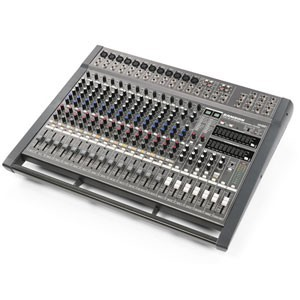
\includegraphics[scale=0.3]{img/mixer.jpg}
   \caption{Mixer Samson con Power TXM20}
   \label{fig:mixer}
\end{figure}

Fuente: \url{http://www.audiomusica.com/catalogo/1088053-txm20-mixer-con-power-samson.html}

\subsubsection*{Caja acústica pasiva DAS DR-115 15''}

\begin{table}[htb!]
\centering
\begin{tabular}{|l|l|}
\hline
Dimensión & 71cm x 46cm x 42cm\\
Peso & 18.6 kg\\
Salida & Speakon\\
Entrada & Speakon \\
Potencia & 350 W \\
Diámetro & 15'' \\
\hline
\end{tabular}
\caption{Ficha Técnica Caja acústica pasiva DAS DR-115 15''}
\end{table}

\begin{figure}[h!t]
   \centering
  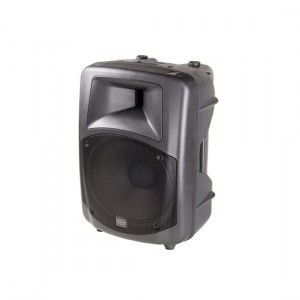
\includegraphics[scale=0.3]{img/caja-acustica.jpg}
   \caption{Caja acústica pasiva DAS DR-115 15''}
   \label{fig:cajaacustica}
\end{figure}
Fuente: \url{http://www.audiomusica.com/catalogo/1070230-dr115-caja-acustica-pasiva-15--das.html}

\newpage
\subsubsection*{Multipar 8x4 PSP-12100 Climb}

\begin{table}[htb!]
\centering
\begin{tabular}{|l|l|}
\hline
Longitud & 30 mts\\
Conexiones & 8 XLR x 4 plug de retorno \\
Cantidad de conexiones & 12 conexiones \\
\hline
\end{tabular}
\caption{Ficha Técnica Multipar 8x4 PSP-12100 Climb}
\end{table}

\begin{figure}[h!t]
   \centering
  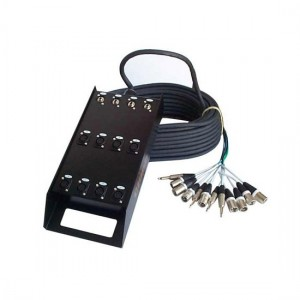
\includegraphics[scale=0.3]{img/multipar.jpg}
   \caption{Multipar 8x4 PSP-12100 Climb}
   \label{fig:multipar}
\end{figure}

\subsubsection*{Interfaz de Audio Profire 2626 M-Audio}

\begin{table}[htb!]
\centering
\begin{tabular}{|l|l|}
\hline
Serie & Profire 2626 \\
Resolución & Hasta 24 bits/192kHz \\
PHantom Power & Si \\
Conexiones de Salida & Firewire \\
Conexiones de Entrada & Firewire \\
Canales de Salida & 8 canales\\
Canales de Entrada & 8 canales\\
\hline
\end{tabular}
\caption{Ficha Técnica Interfaz de Audio Profire 2626 M-Audio}
\end{table}

\begin{figure}[h!t]
   \centering
  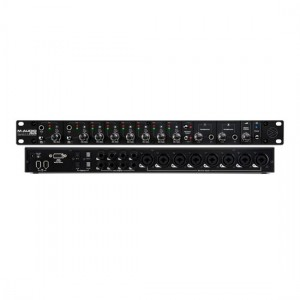
\includegraphics[scale=0.3]{img/interfaz.jpg}
   \caption{Interfaz de Audio Profire 2626 M-Audio}
   \label{fig:interfaz}
\end{figure}
Fuente: \url{http://www.audiomusica.com/catalogo/1091807-profire2626-interface-maudio.html}

\subsubsection*{Monitor de Estudio Mediaone Activo Samson}

\begin{table}[htb!]
\centering
\begin{tabular}{|l|l|}
\hline
Rango de Frecuencia & 50 Hz - 23 kHz \\
Potencia & 2x20 watts RMS \\
Medida parlante & 5 pulgadas \\
\hline
\end{tabular}
\caption{Ficha Técnica Monitor de Estudio Mediaone Activo Samson}
\end{table}

\begin{figure}[h!t]
   \centering
  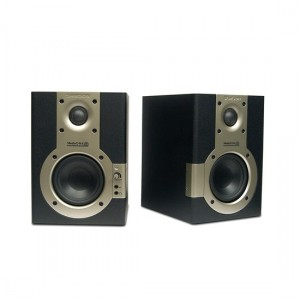
\includegraphics[scale=0.3]{img/monitor.jpg}
   \caption{Monitor de Estudio Mediaone Activo Samson}
   \label{fig:monitor}
\end{figure}

Fuente \url{http://www.audiomusica.com/catalogo/1091348-mediaone-5a-monitor-activo-par-samson.html}

\subsubsection*{Ecualizador Gráfico SR231QXV 2x31 DOD-EU}

\begin{table}[htb!]
\centering
\begin{tabular}{|l|l|}
\hline
Cantidad de Bandas & 31 bandas stereo \\
Serie & SR231QXV \\
Tipo de Salida & XLR - Jack 1/4 pulgada \\
Tipo de Salida & XLR - Jack 1/4 pulgada \\
\hline
\end{tabular}
\caption{Ficha Técnica Ecualizador Gráfico SR231QXV 2x31 DOD-EU}
\end{table}

\begin{figure}[h!t]
   \centering
  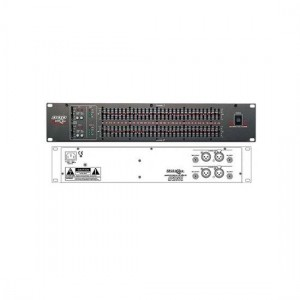
\includegraphics[scale=0.3]{img/ecu.jpg}
   \caption{Ecualizador Gráfico SR231QXV 2x31 DOD-EU}
   \label{fig:ecu}
\end{figure}

Fuente: \url{http://www.audiomusica.com/catalogo/1033860-sr231qxv-ecualiz-grafico-2-x-31-dod--eu.html}

\newpage
\subsubsection*{Computador HP AIO G1-2012LA}

\begin{table}[htb!]
\centering
\begin{tabular}{|l|l|}
\hline
Procesador (CPU) &AMD Dual-Core E350 1.6GHz 1MB L2 (núcleo Bobcat) \\
Número de núcleos & 2 \\
Gráficos (GPU) & AMD HD6310 (80 processors, 500Mhz), Integrado en la CPU \\
Chip Placa Madre (FCH) &  Hudson \\
Plataforma & Brazos (CPU+GPU+FCH) -Zacate (CPU+GPU), construido en 40nm \\ 
Consumo & 18W (CPU+GPU), 5W (FCH) \\
Pantalla & Pantalla LCD ancha HD de 20'', 16:9 \\
Memoria & 2GB DDR3 1333MHz PC3-10600 (1x2GB) \\
Disco Duro & 500GB 7200rpm - SATA - 3.0 Gb/sec \\
Unidad Óptica & Grabadora de DVD SuperMulti con tecnología LightScribe(6d)\\
Audio & Altavoces 2.0 de alto rendimiento \\
Interfaz de Red & 10/100Base-T \\
WiFi & 802.11b/g/n \\
Dimensiones & 50.2 x 20.0 x 36.6 (cm) \\
Peso & 6.1 Kg \\
\hline
\end{tabular}
\caption{Ficha Técnica Computador HP AIO G1-2012LA}
\end{table}

\begin{figure}[h!t]
   \centering
  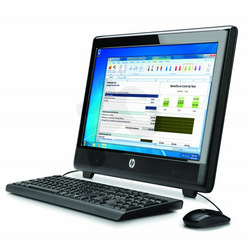
\includegraphics[scale=0.3]{img/computador.jpg}
   \caption{Computador HP AIO G1-2012LA}
   \label{fig:computador}
\end{figure}

Fuente: \url{http://www.pcfactory.cl/producto/9216-AIO.G1-2012LA.AMD.Dual-Core.E350.2Gb.500Gb.20.WiFi.DVDRW.W7St}
\newpage
\subsubsection*{Tarjeta de Sonido Delta 66 M-AUDIO}

\begin{table}[htb!]
\centering
\begin{tabular}{|l|l|}
\hline
Resolución & 24 bits/92 kHz \\
Phantom Power & No \\
Conexiones de Salida & 1/4 TRS\\
Conexiones de Entrada & 1/4 TRS\\
Canales de Salida & 6 salidas\\
Canales de Entrada & 6 entradas\\
Serie & Delta \\
\hline
\end{tabular}
\caption{Ficha Técnica Tarjeta de Sonido Delta 66 M-AUDIO}
\end{table}

\begin{figure}[h!t]
   \centering
  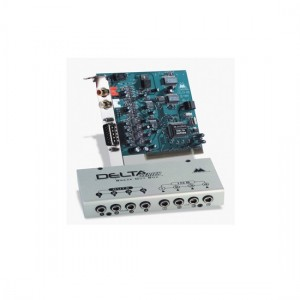
\includegraphics[scale=0.5]{img/tarjetasonido.jpg}
   \caption{Tarjeta de Sonido Delta 66 M-AUDIO}
   \label{fig:tarjetasonido}
\end{figure}

Fuente: \url{http://www.audiomusica.com/catalogo/1008410-delta-66-tarjeta-audio-maudio.html}

\subsubsection*{Software Protools M-POWERED M-AUDIO}

\begin{table}[htb!]
\centering
\begin{tabular}{|l|l|}
\hline
Versión & 8 \\
Número máximo de pistas MIDI & 256 pistas \\
Número máximo de pistas de Audio & 32 pistas \\
\hline
\end{tabular}
\caption{Ficha Técnica Software Protools M-POWERED M-AUDIO}
\end{table}

\newpage
\begin{figure}[h!t]
   \centering
  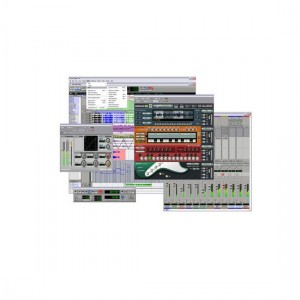
\includegraphics[scale=0.6]{img/protools.jpg}
   \caption{Software Protools M-POWERED M-AUDIO}
   \label{fig:protools}
\end{figure}

Fuente: \url{http://www.audiomusica.com/catalogo/1085701-protools-mpowered-software-maudio.html}
